\section{Discussion}\label{sec:dis}


% From \autoref{tab:afrho} we can conclude that the comet C/2019 L3 is very active due to its high $A(0)f\rho$ values during the observational run, while C/2020 P3 is less active since its $A(0)f\rho$ values are only about {\SI{10}{\percent}} of that of C/2019 L3. 
Based on the data presented in Table~\ref{tab:afrho}, it can be inferred that the comet C/2019 L3 exhibited a high level of activity during the observation period, as indicated by its significantly higher $A(0)f\rho$ values compared to C/2020 P3. In contrast, the $A(0)f\rho$ values of C/2020 P3 were only about \SI{10}{\percent} of those of C/2019 L3. 
Comparing $A(0)f\rho$ values with that of other LPCs, just as Fig.~\ref{fig:afrho-ref} shown, C/2019 L3 is very active at heliocentric distance of $\thicksim${\SI{4}{\astronomicalunit}}, and C/2020 P3 is moderately active at heliocentric distance of $\thicksim${\SI{7}{\astronomicalunit}}. 
\st{Moreover, the R-band $A(0)f\rho$ values in the reference aperture of {\SI{e4}{\km}} appear a slight decrese in trend as it approached to perihelion viewed from Fig.~\ref{fig:a0frho-c2019}, so it seems that the heat of the Sun plays a minor role on the activity of C/2019 L3 during the observational period.} \ul{Moreover, the $A(0)f\rho$ values of C/2019 L3 in the R-band for the reference aperture of {\SI{e4}{\km}} exhibit a slight decreasing trend as the comet approached perihelion, as shown in Fig.~\ref{fig:a0frho-c2019}. This suggests an abnormal activity of the comet. }% 在此只写活动性显现出异常, 不作过度猜测
On the other hand, 
the BC-band $A(0)f\rho$ of C/2019 L3 up to \SI{24710 +- 125}{\cm} on \DTMdate{2022-1-19} posted on The Astronomer's Telegram\footnote{\href{https://www.astronomerstelegram.org/?read=15186}{https://www.astronomerstelegram.org/?read=15186}}, with heliocentric distance $r = \SI{3.56}{\astronomicalunit}$ and geocentric distance $\Delta = \SI{2.61}{\astronomicalunit}$, indicates that C/2019 L3 appears very active near the perihelion. 


% 与其他LPC比较,相位角均校正至0
\begin{figure}
    \centering
    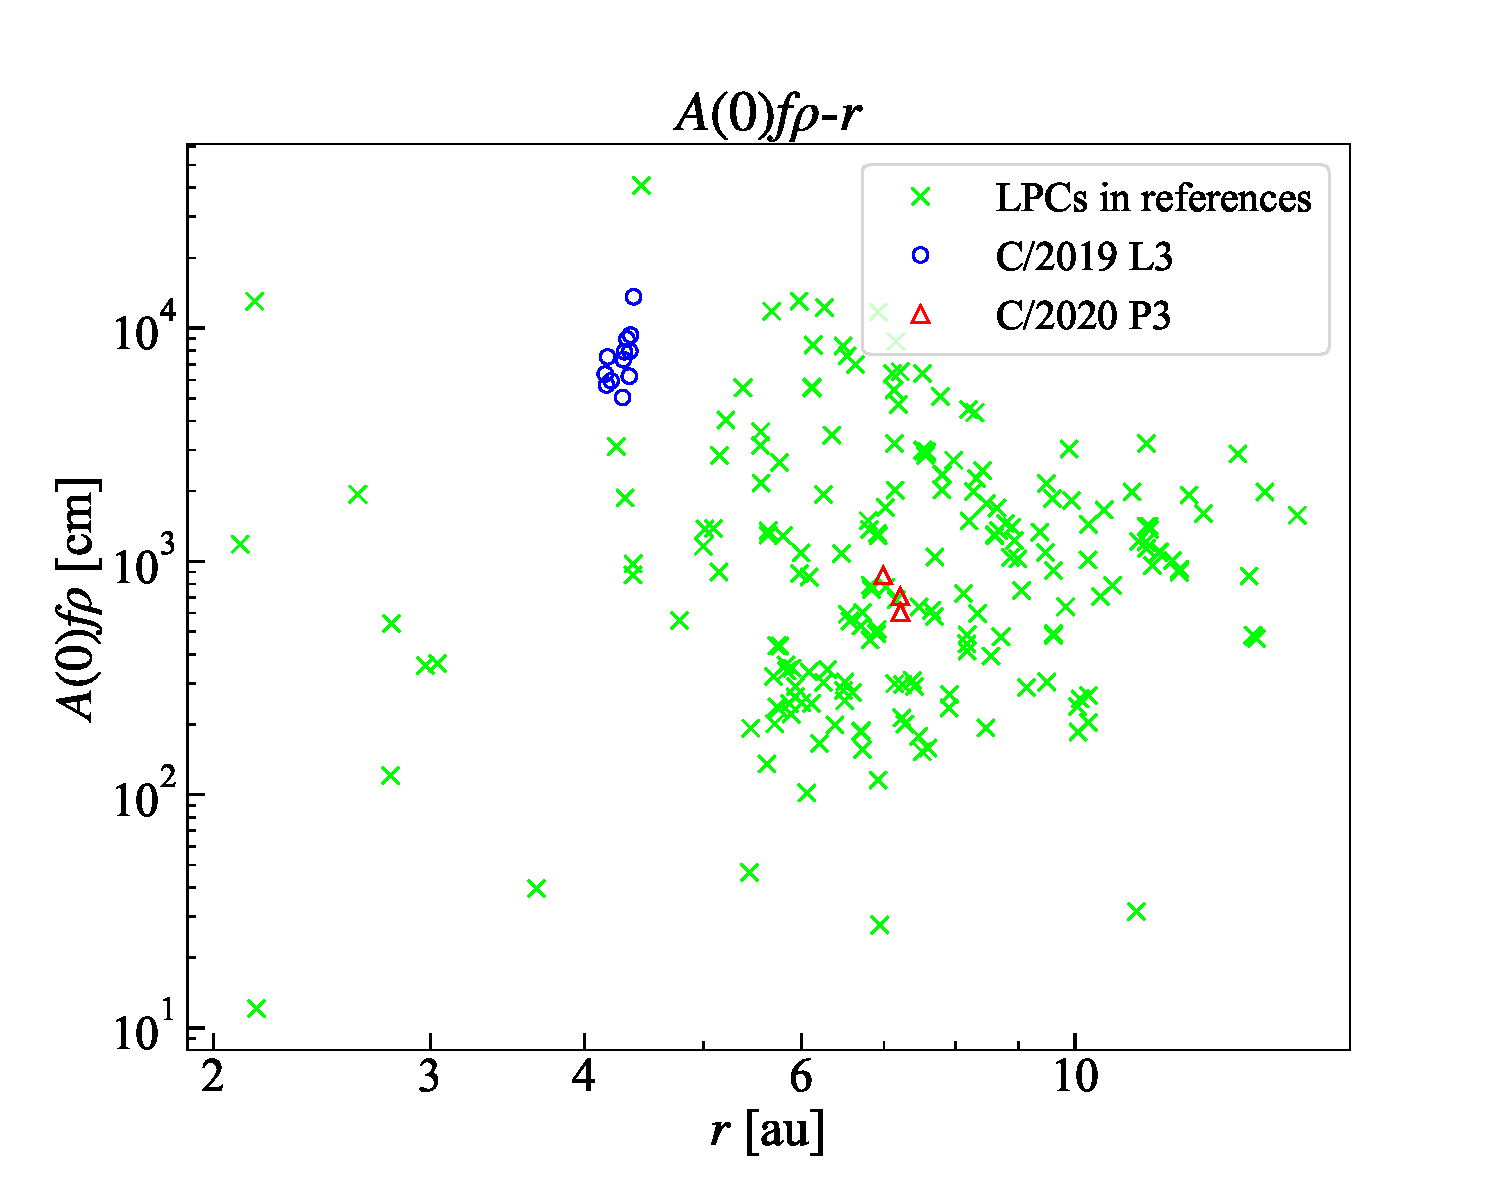
\includegraphics[width=\columnwidth]{a0frho-r.pdf}
    \caption{$A(0)f\rho$ values measured in this work compared with that of other LPCs in  literature by \citet{mazzotta_epifani_observational_2014}, \citet{garcia_photometry_2021}, \citet{garcia_observational_2020}, \citet{rousselot_monitoring_2014}, \citet{meech_activity_2009}, \citet{sarneczky_activity_2016}, \citet{solontoi_ensemble_2012}, \citet{szabo_spectrophotometry_2002}. All data have been adjusted to phase angle \ang{0}. }\label{fig:afrho-ref}
\end{figure}% data amount error

\begin{figure}
    \centering
    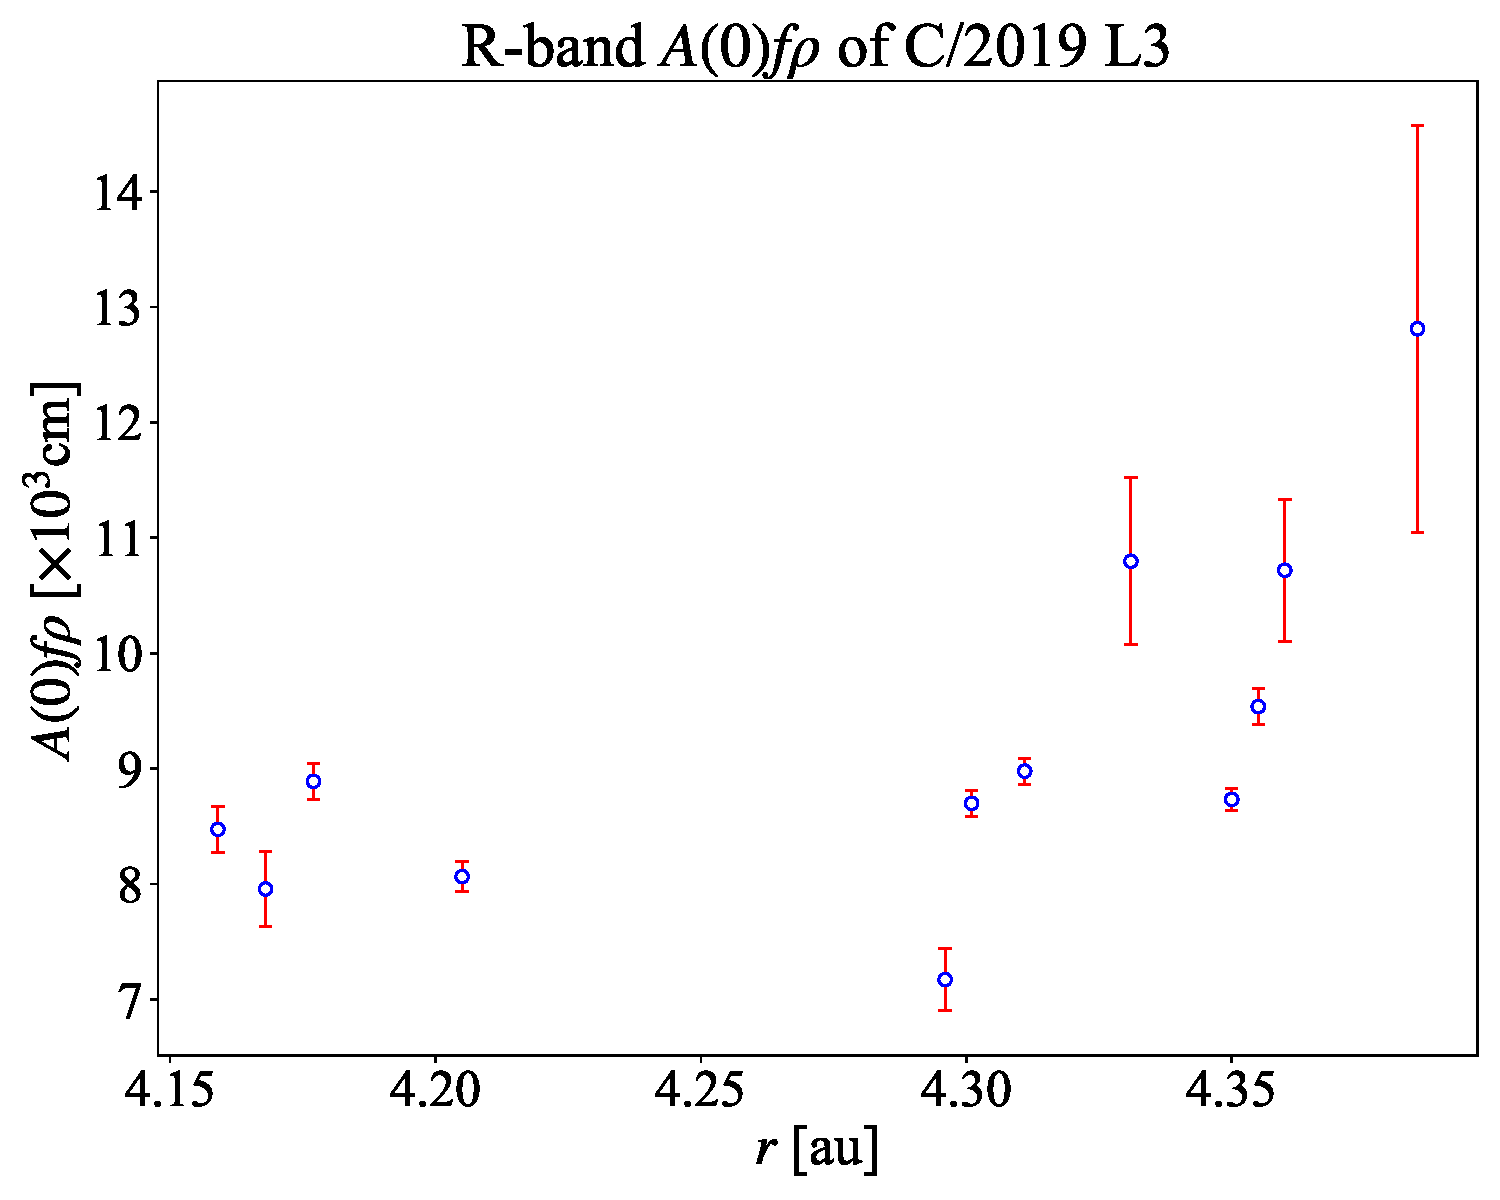
\includegraphics[width=\columnwidth]{a0frho-r-C2019L3.pdf}
    \caption{R-band $A(0)f\rho$ values of C/2019 L3 as a function of heliocentric distance. }\label{fig:a0frho-c2019}
\end{figure}

According to the study by \cite{ramirez_ubvric_2012}, the solar colors are as follows: 
${(\mathrm{B} - \mathrm{V})}_{\odot} = \num{0.653 +- 0.005}$, 
${(\mathrm{V} - \mathrm{R})}_{\odot} = \num{0.352 +- 0.007}$, and 
${(\mathrm{R} - \mathrm{I})}_{\odot} = \num{0.350 +- 0.009}$. 
The average color indices of two Long-period comets and three dynamically new comets were calculated by \cite{meech_activity_2009} to be 
$\langle \mathrm{B} - \mathrm{V} \rangle = \num{0.76 +- 0.01}$ and 
$\langle \mathrm{V} - \mathrm{R} \rangle = \num{0.43 +- 0.01}$, 
with their heliocentric distances ranging from \SIrange{5.8}{14.0}{\astronomicalunit}. 
\cite{solontoi_ensemble_2012} studied six Long-period comets within \SI{5}{\astronomicalunit} of the Sun and obtained the average color indices of 
$\langle \mathrm{B} - \mathrm{V} \rangle = \num{0.687 +- 0.005}$ and 
$\langle \mathrm{V} - \mathrm{R} \rangle = \num{0.443 +- 0.003}$. 
\cite{jewittCOLORSYSTEMATICSCOMETS2015} investigated Long-period comets with large range of heliocentric distances (\SIrange{1.875}{17.982}{\astronomicalunit}), and the average color indices were found to be 
$\langle \mathrm{B} - \mathrm{V} \rangle = \num{0.78 +- 0.02}$, 
$\langle \mathrm{V} - \mathrm{R} \rangle = \num{0.47 +- 0.02}$, and 
$\langle \mathrm{R} - \mathrm{I} \rangle = \num{0.42 +- 0.03}$. 

Fig.~\ref{fig:color_index}a is the color indices $\mathrm{B}-\mathrm{V}$, $\mathrm{V}-\mathrm{R}$, and $\mathrm{R}-\mathrm{I}$ of C/2019 L3 as a function of heliocentric distance in \si{\astronomicalunit}, all exhibiting variability during the approach to perihelion. 
As C/2019 L3 approached perihelion, its $\mathrm{V}-\mathrm{R}$ color index showed a tendency towards blue. 
Considering its position at a heliocentric distance of about {\SI{4}{\astronomicalunit}}, with a temperature of around {\SI{140}{\K}}, the gas-driven effects are significant. 

Fig.~\ref{fig:color_index}b is the $\langle \mathrm{B}-\mathrm{V} \rangle$ versus $\langle \mathrm{V}-\mathrm{R} \rangle$ plot of C/2019 L3, C/2020 P3 and other LPCs. 
The color index of the Sun \citep{ramirez_ubvric_2012} is marked as a red circle with dot. 
As we can see, the $\langle \mathrm{B} - \mathrm{V} \rangle$ colors of two comets are redder than the Sun, while the $\langle \mathrm{V} - \mathrm{R} \rangle$ colors of them are bluer than the Sun. 
Compared with LPCs in other works, the $\langle \mathrm{B} - \mathrm{V} \rangle$ color of C/2019 L3 is consistent with them, while the $\langle \mathrm{V} - \mathrm{R} \rangle$ color of C/2019 L3 is significantly bluer than them. For C/2020 P3, the $\langle \mathrm{B} - \mathrm{V} \rangle$ color is redder while the $\langle \mathrm{V} - \mathrm{R} \rangle$ color is bluer. 
In general, the color indices of the two LPCs studied in this work differ from those of other LPCs. 

The reddening of C/2019 L3 on each observation date is shown in Fig.~\ref{fig:reddening}, with the blue dotted line indicating the mean value. The plot reveals that over the observation course of nearly two months, C/2019 L3 exhibited multiple transitions from a reddish to a bluish color, possibly due to variations in the composition of the coma \citep{ivanova_colour_2017}.

% V-R随日心距呈现变蓝的趋势, 在4au左右CO2的升华作用较明显, 因此, C/2019 L3的活动性可能是由于CO2的升华导致

\begin{figure}
    \centering
    \subcaptionbox{Color indices vs.\ heliocentric distance for C/2019 L3}{
        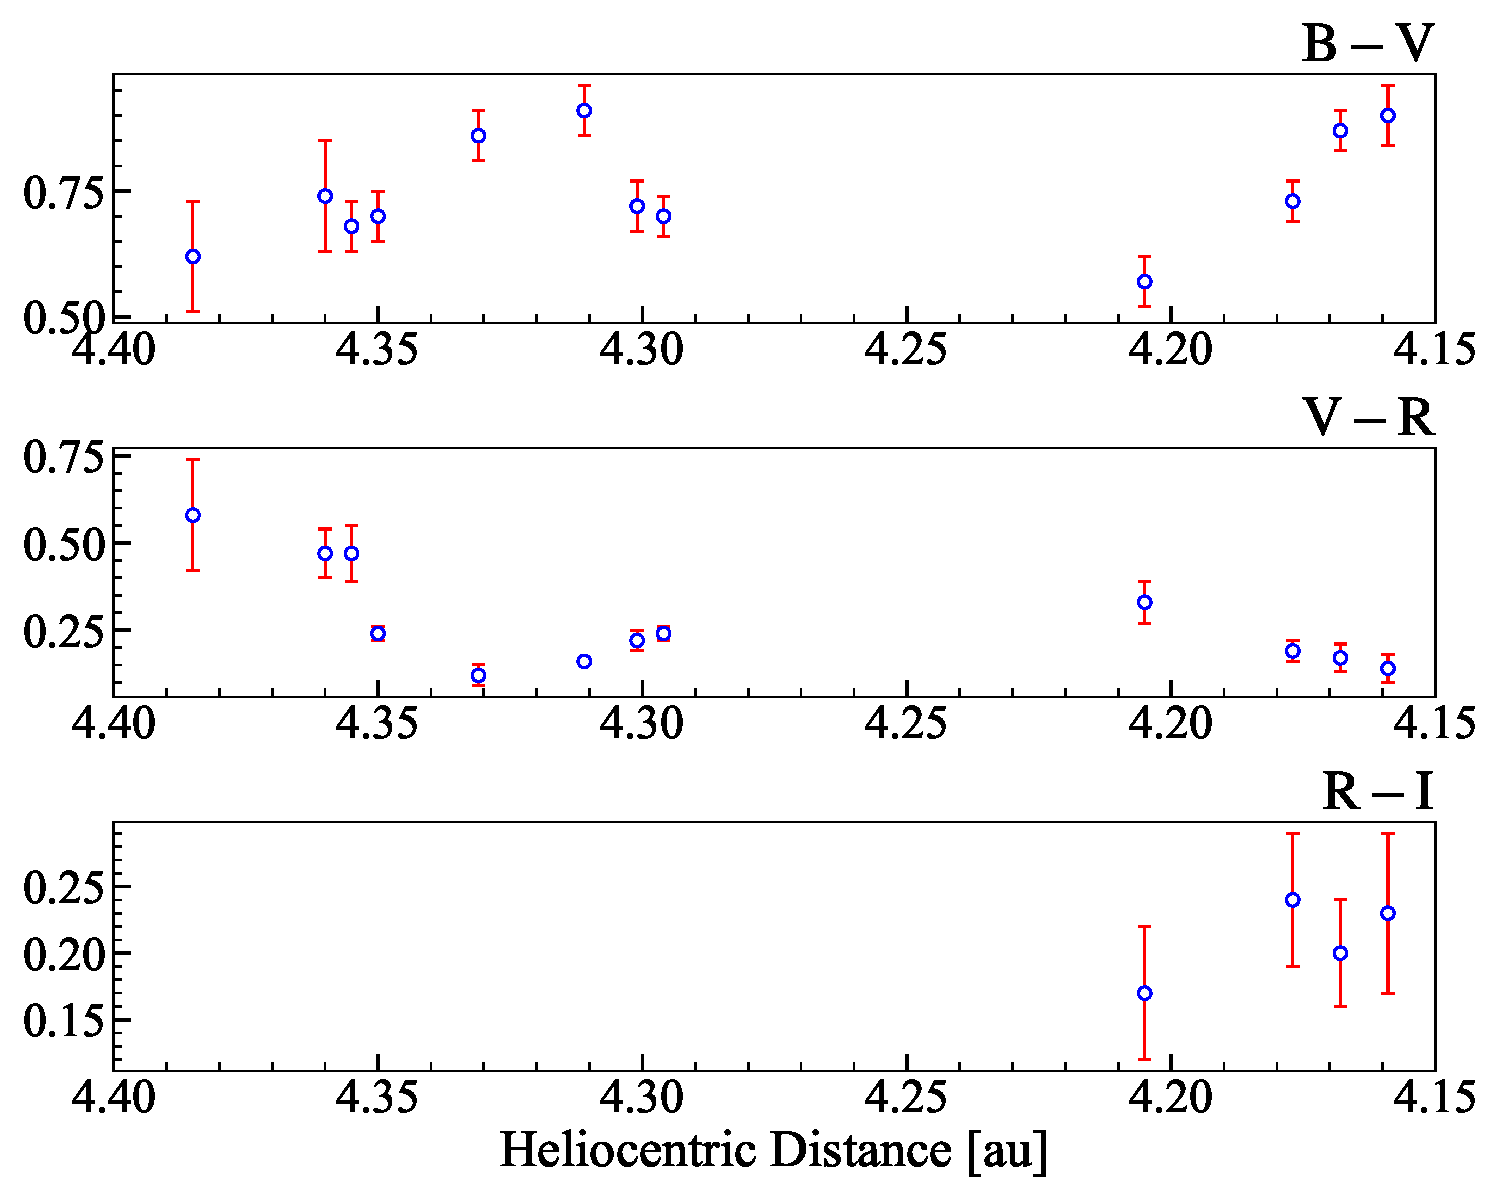
\includegraphics[width=\linewidth]{color-r.pdf} 
    }
    \subcaptionbox{Color indices $\langle \mathrm{B} - \mathrm{V} \rangle$ vs. $\langle \mathrm{V} - \mathrm{R} \rangle$ plot of Long-period comets}{
        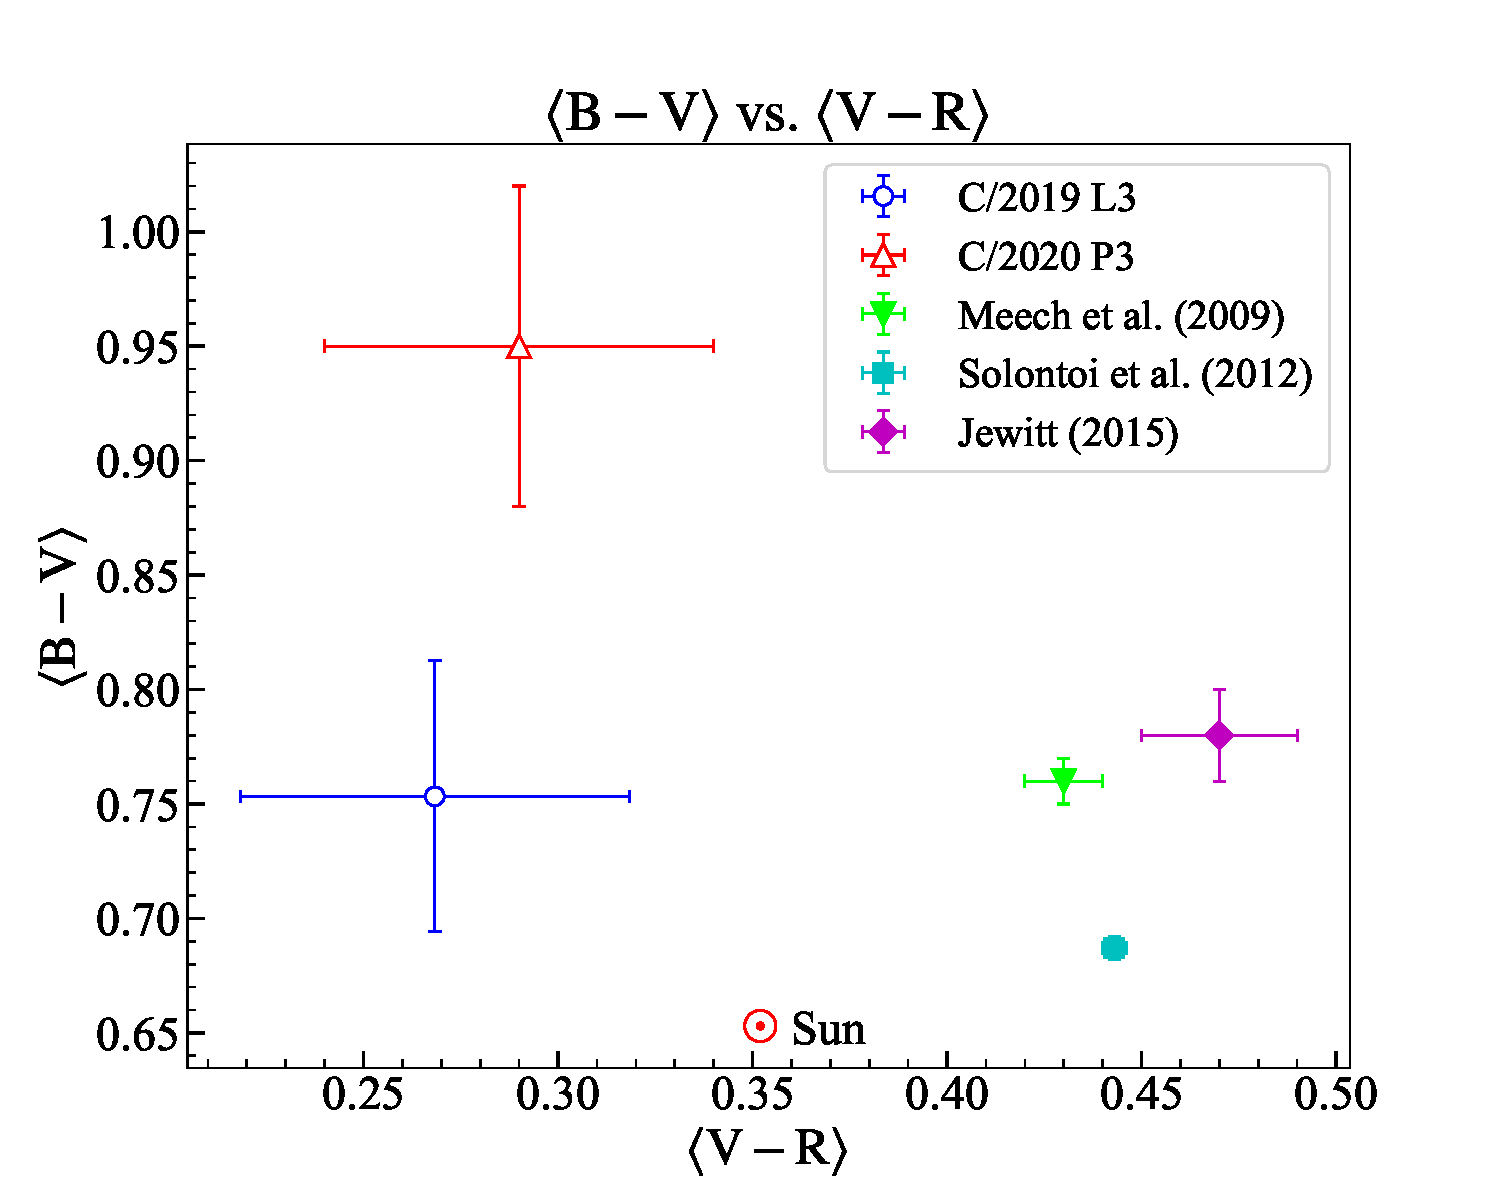
\includegraphics[width=\linewidth]{color-color.pdf}
    }
   
    \caption{Color index plot \ul{of C/2019 L3, C/2020 P3 and other Long-period comets.} }\label{fig:color_index}
\end{figure}


